\section{Backup}

\begin{frame}
    \frametitle{Pressione ed isoterme}
    \framesubtitle{}
  
    \begin{columns}
        \begin{column}{0.5\textwidth}
          $$
          p\,=\,\frac{k_BT}{\lambda_T^3}g_{5/2}\left(z\right)\,-\,\frac{k_BT}{V}\log{\left(1\,-\,z\right)}
          $$
          \vspace{12pt}
          \begin{itemize}[itemsep=0.5em, label=$\bullet$]
            \item curva limitante per isoterme è $pV^{5/3}\,=\,const$
            \item parallelismo con Van der Waals
          \end{itemize}
        \end{column}
        
        \begin{column}{0.5\textwidth}
          \begin{figure}
              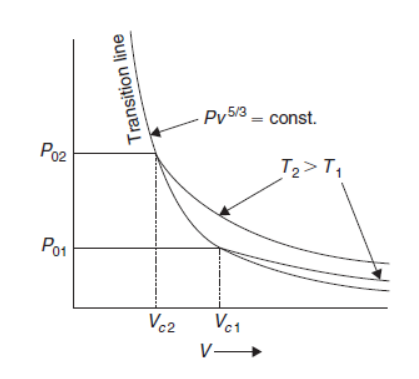
\includegraphics[width=0.8\textwidth]{Immagini/isoBose.png}
              \caption{Isoterme del gas di Bose ideale}
          \end{figure}
        \end{column}
      \end{columns}
  
  \end{frame}